\documentclass[a4paper, 11pt]{article} % Font size (can be 10pt, 11pt or 12pt) 

\usepackage[protrusion=true,expansion=true]{microtype} % Better typography
\usepackage{graphicx} % Required for including pictures
\usepackage{wrapfig} % Allows in-line images
\usepackage{hyperref}
\usepackage{mathpazo} % Use the Palatino font
\usepackage[utf8]{inputenc}

\usepackage{listings}
\usepackage{xcolor}
\definecolor{bluekeywords}{rgb}{0.13,0.13,1}
\definecolor{greencomments}{rgb}{0,0.5,0}
\definecolor{redstrings}{rgb}{0.9,0,0}
\lstset{language=[Sharp]C,
	showspaces=false,
	showtabs=false,
	breaklines=true,
	showstringspaces=false,
	breakatwhitespace=true,
	escapeinside={(*@}{@*)},
	commentstyle=\color{greencomments},
	keywordstyle=\color{bluekeywords},
	stringstyle=\color{redstrings},
	basicstyle=\ttfamily
}


\linespread{1.05} % Change line spacing here, Palatino benefits from a slight increase by default

\makeatletter
\renewcommand\@biblabel[1]{\textbf{#1.}} % Change the square brackets for each bibliography item from '[1]' to '1.'
\renewcommand{\@listI}{\itemsep=0pt} % Reduce the space between items in the itemize and enumerate environments and the bibliography

\renewcommand{\maketitle}{ % Customize the title - do not edit title and author name here, see the TITLE block below
\begin{flushright} % Right align
{\LARGE\@title} % Increase the font size of the title

\vspace{50pt} % Some vertical space between the title and author name

{\large\@author} % Author name
\\\@date % Date

\vspace{40pt} % Some vertical space between the author block and abstract
\end{flushright}
}

%----------------------------------------------------------------------------------------
%	TITLE
%----------------------------------------------------------------------------------------

\title{\textbf{Laboratorio di Applicazioni Mobili}\\ % Title
RoadSoSecurity} % Subtitle

\author{\textsc{Bartolomeo Lombardi} % Author
\\{\textit{Universita' degli studi di Bologna}}} % Institution

\date{\today} % Date

%----------------------------------------------------------------------------------------

\begin{document}

\maketitle % Print the title section

%----------------------------------------------------------------------------------------
%	ABSTRACT AND KEYWORDS
%----------------------------------------------------------------------------------------

%\renewcommand{\abstractname}{Summary} % Uncomment to change the name of the abstract to something else

\begin{abstract}
Le condizioni del manto stradale possono causare seri incidenti, spesso con tragiche conseguenze; secondo l'Istat nel 2016 si sono verificati in Italia 175.791 incidenti stradali con lesioni a persone che hanno provocato 3.283 vittime e 249.175 feriti. La presenza degli smartphone fornisce una nuova piattaforma su cui implementare reti di sensori, sistemi di assistenza ai guidatori e altre applicazioni intelligenti di trasporto (ITS). In questo lavoro di progetto l'attenzione si è posta sul monitoraggio di buche stradali e del rilevamento di indicendi in maniera del tutto automatica, attraverso la sensoristica di base.
\end{abstract}

\vspace{30pt} % Some vertical space between the abstract and first section

%----------------------------------------------------------------------------------------
%	ESSAY BODY
%----------------------------------------------------------------------------------------

\section{Introduzione}
Le condizioni del manto stradale sono state identificate da organizzazioni internazionali come una delle principali cause di incidenti nel mondo. Infatti, studi mostrano che le condizioni dinamiche della strada possono provocare comportamenti imprevedibili da parte dei guidatori e deterioamenti di parti meccaniche del veicolo, i quali possono avere un forte impatto economico. Sviluppare una mappa delle condizioni stradali può avere un riscontro positivo sulla sicurezza dei conducenti e dei pedoni. 

Quindi si è posto come obiettivo di sviluppare un'applicazione Android che utilizzi i sensori dello smartphone, ovvero GPS e accelerometro per rilevare automaticamente:
\begin{itemize}
	
	\item \textbf{Anomalie stradali (buche)} \\
	Facendo uso dell'accelerometro, si è implementato un sistema smartphone-based capace di rilevare lo sbalzo sull'asse Z e salvare la posizione dell’anomalia attraverso il GPS (in remoto esponendo un servizio web). Le anomalie sono mostrate all’utente attraverso l’applicativo con dei marker posizionati sulla mappa. Inoltre se la posizione corrente del conducente è in un raggio di 6 metri dall’anomalia, allora un alert acustico avvertirà l'utente della presenza \cite{Mohamed2016}.
	
	\item \textbf{Incidenti con l'invio automatico di SMS} \\
	Anche in questo caso facendo uso dell'accelerometro si è rilevato lo sbalzo sull’asse X che un veicolo durante l’urto subisce, nel caso di un incidente verrà inviato automaticamente un SMS al numero che l'utente ha scelto precedentemente \cite{Faiz2016}.
	
\end{itemize} 
La logica dell'applicativo è stata completamente distribuita sul back-end, in modo tale da lasciare allo smartphone la rilevazione e l'analisi dei dati dai sensori per individuare le anomalie. 
 
\section{Tecnologie utilizzate}
In questo paragrafo verranno brevemente descritte le principali tecnologie utilizzate durante la realizzazione del progetto:

\begin{itemize}
	\item Android SDK (Software Development Kit) è un pacchetto di sviluppo per applicazioni che contiene un set completo di API (Application Programming Interface), librerie e strumenti di sviluppo utili a compilare, testare e debug-gare applicazioni per Android.
	
	\item Microsoft ASP.NET MVC Framework 4.5  è un tipo di Model-View-Controller sviluppato da Microsoft come aggiunta ad ASP.NET, offrendo un'alternativa al modello ASP.NET Web Forms, che viene utilizzato per la creazione di applicazioni web. Esso consente di separare la logica dell’interfaccia dal tipo di applicazione che si sta sviluppando, dividendola in tre componenti distinti: Model (modello), che contiene i dati e fornisce i metodi per accedervi; se l’applicazione utilizza un database, la progettazione del modello è guidata dalle tabelle della base di dati; View (vista), che visualizza i dati contenuti nel Model; Controller (controllo), che si occupa delle iterazioni con l’utente invocando i metodi presenti nel Model e cambiando l’output dell’interfaccia tramite il View.
	
	\item Database SQL Server 2012 è un DBMS relazionale (Relational Database Management System RDBMS), prodotto da Microsoft. Microsoft SQL Server usa una variante del linguaggio SQL standard (lo standard ISO certificato nel 1992) chiamata "Transact-SQL" (T-SQL).
\end{itemize}

\section{Back-end}
Il sistema è stato progettato in modo distribuito su due entità principali: l'applicativo Android e un server back-end sviluppato in $C\#$. Come già citato in precedenza, l'applicazione utilizza le letture dall'accelerometro e dal GPS dello smartphone per eseguire l'individuazione automatica di anomalie stradali ed eventuali incidenti. L'output delle funzioni dell'applicativo mobile sono le anomalie rilevate insieme alle loro posizioni, quest'ultime vengono poi trasmesse al server attraverso chiamate esplicite dei metodi HTTP, come è possibile intuire nello schema in Figura \ref{fig:rest}.

\begin{figure}[h]
	\begin{center}
		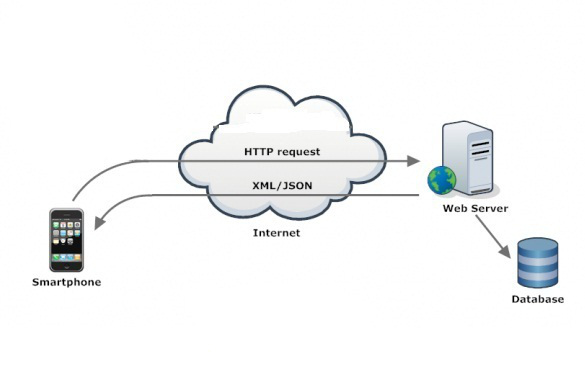
\includegraphics[width=\textwidth]{images/rest.jpg}
	\end{center}
	\caption{Web Service RESTful}
	\label{fig:rest}
\end{figure}

 Dato che il manto stradale è in continuo cambiamento, le anomalie possono essere riparate, quindi si è pensato di associare ad ogni anomalia un livello di fiducia; l'algoritmo che si occupa della gestione di tale parametro è contenuto nel server: in grado di aumentare il valore nel caso in cui l'anomalia venga rilevata più volte, oppure decrementato se non viene riportata per un lungo periodo di tempo. E' stata implementata questa funzione al fine di individuare gli interventi di manutenzione che risolvono le anomalie stradali.

Si è optato per un Web Service con uno stile architetturale di tipo RESTful (Figura \ref{fig:rest}) sviluppato con tecnologie Microsoft, attualmente hostato su \url{www.myASP.net} per un periodo gratuito di sessanta giorni. 
Attraverso l'uso del metodo GET si sono esposte due risorse:

\begin{enumerate}
	\item \url{http://bartlombardi-001-site1.dtempurl.com/Api/Anomalies}
	\item \url{http://bartlombardi-001-site1.dtempurl.com/api/Anomalies?latitude=0.931196&longitude=4.4482012}
\end{enumerate}
La risorsa 1 offre un output di tutte le anomalie che sono state rilevate dagli utenti, formattate in JSON, mentre la 2 inserisce l'anomalia nella base di dati, dopo aver effettuato alcuni controlli che descriveremo successivamente. Per salvare i dati si è pensato di creare un piccolo database con una semplice tabella, poichè gli oggetti da salvare erano dello stesso tipo e quindi con le stesse proprietà, infatti una anomalia è stata mappata come un oggetto avente le seguenti proprietà:
\begin{itemize}
	\item Latitude: rappresenta la coordinata geografica della latitudine
	\item Longitude: rappresenta la coordinata geografica della longitudine
	\item FlagAnomaly: un flag per rendere visibile l'anomalia, utile per il front-end
	\item Trust: il valore di fedeltà
	\item Count: il numero di volte che è stata rilevata tale anomalia
	\item Date: la data di rilevazione dell'anomalia
	\item Update: la data di aggiornamento dell'anomalia
\end{itemize}
La creazione della tabella all'interno del database si è ottenuta attraverso l'esecuzione nella console dello script .sql nel provider dove è stato caricato il web service, poichè fornisce servizi di tipo Database SQL Server 2012.
\begin{verbatim}
CREATE TABLE [dbo].[Anomalies] 
(
    [Id]          INT        IDENTITY (1, 1) NOT NULL,
    [Latitude]    FLOAT (53) NOT NULL,
    [Longitude]   FLOAT (53) NOT NULL,
    [FlagAnomaly] BIT        NOT NULL,
    [Trust]       FLOAT (53) NOT NULL,
    [Count]       INT        NOT NULL,
    [Date]        DATETIME   NOT NULL,
    [Update]      DATETIME   NOT NULL,
    PRIMARY KEY CLUSTERED ([Id] ASC)
);
\end{verbatim}
Una volta creato il database e collegato al web server attraverso la connection string contenuta nel file Web.confing, si sono sviluppati due metodi GET per esporre le risorse, come descritto in precedenza. La classe che si è occupata della gestione dei dati è \textit{DataController}, infatti la funzione \textit{getAllAnomaly()} restituisce tutte le anomalie contenute nel database, mentre la funzione chiamata dal secondo metodo GET \textit{addAnomaly(latitude, longitude)} inserisce la nuova anomalia nella banca dati. Di seugito viene riportato la parte di codice per esporre le risorse attraverso il metodo GET.
\begin{lstlisting}
public IEnumerable<Anomaly> Get() { 
  return DataController.getAllAnomaly(); 
}
public void Get(double latitude, double longitude) {
  DataController.addAnomaly(latitude, longitude);
}
\end{lstlisting}
La funzione \textit{getAllAnomaly()} è banale in quanto crea una lista di tipo Anomaly che viene semplicemente mappata con la lista degli oggetti anomalies contenuti nel database.

\begin{lstlisting}
public List<Anomaly> getAllAnomaly() {   
  List<Anomaly> result = new List<Anomaly>();
  result = AnomalyDb.anomalies.ToList();

  return result;
}
\end{lstlisting}
L'output di tale risorsa (\url{http://bartlombardi-001-site1.dtempurl.com/Api/Anomalies}) è una lista di anomalie con le proprietà descritte precedentemente, formattate in JSON per avere una maggiore semplicità di manipolazione da parte del front-end, di seguito viene riportato una parte dell'output.
\begin{verbatim}
[
  ...
  {
    "Id": 22,
    "Latitude": 0.931196,
    "Longitude": 4.4482012,
    "FlagAnomaly": true,
    "Trust": 71.4,
    "Count": 2,
    "Date": "2017-08-30T17:02:36.14",
    "Update": "2017-08-30T17:02:36.14"
  },
  ...
]
\end{verbatim}
Per quanto riguarda invece la funzione \textit{addAnomaly(double latitude, double longitude)} del \textit{DataController} è un pò più articolata, in quanto prima di inserire una nuova anomalia nella base di dati, controlla se è gia contenuta; nel caso in cui lo fosse, aggiorna semplicemente: il count a più 1, il valore di fedeltà attuale viene aggiornato, rafforzandone l'esistenza secondo l'equazione $New\_Trust = (new\_Count * 0.7) + old\_Trust$, viene aggiornata la data di rilevazione e di aggiornamento. 

\begin{lstlisting}
public void addAnomaly(double latitude, double longitude)
{
  List<Anomaly> allAnomaly = getAllAnomaly();
  bool isEntered = false;

  foreach (Anomaly a in allAnomaly)
  {
    if (Math.Abs(a.Latitude - latitude) <= Double.Epsilon && Math.Abs(a.Longitude - longitude) <= Double.Epsilon)
    {
      isEntered = true;
      a.FlagAnomaly = true;
      a.Count += 1;
      a.Trust = (a.Count * 0.7) + a.Trust;
      a.Date = DateTime.Now;
      a.Update = DateTime.Now;
      AnomalyDb.SaveChanges();
    }
  }

  if (!isEntered)
  {
    Anomaly newAnomaly = new Anomaly{ Latitude=latitude, Longitude=longitude, FlagAnomaly=false, Trust=70, Count=1,  Date=DateTime.Now, Update=DateTime.Now };
    AnomalyDb.anomalies.Add(newAnomaly);
    AnomalyDb.SaveChanges();
  }
}
\end{lstlisting}
Dove $old\_Trust$ è il valore di fedeltà del record esistente e $New\_Count$ è il numero di utenti passati da quella posizione e che hanno registrato un rilevamento. Utilizzando questo approccio, se l'anomalia viene rilevata da un certo numero di veicoli, il valore di fedeltà può raggiunge 100, implicando che tale anomalia esiste con una possibilità del $100\%$.
Il caso contrario è quando si rileva una anomalia non presente nella banca dati, allora questa viene aggiunta con un valore iniziale di fedeltà pari al $70\%$, deducendo che l'anomalia ha una probabilità del $70\%$ di esistere.

Avendo un sistema in continuo aggiornamento, può aiutare le autorità a individuare e organizzare per risolvere le anomalie del manto stradale. Le informazioni di ogni anomalia registrata devono essere aggiornate, rinforzando l'esistenza fino a raggiungere il $100\%$ o diminuendo fino al $0\%$ (caso in cui l'anomalia non viene più rilevata e di conseguenza risolta). Questa procedura di aggiornamento viene eseguita regolarmente su tutto il database. Ogni 48 ore, un \textit{Thread} viene svegliato per eseguire un controllo su tutte le voci registrate. La funzionalità principale di tale \textit{Job} è ridurre il valore di fedeltà del $5\%$ dei record che non sono stati rilevati nelle ultime 48. Ogni due giorni, quindi, il punteggio di fedeltà continuerà a diminuire fino a raggiungere il $0\%$, a questo punto l'anomalia verrà eliminata dal database e scomparirà di conseguenza dalla mappa visualizzata dal front-end, implicando che il problema dell'anomalia stradale sia stato risolto. La parte di codice che esegue il \textit{Thread} è la funzione seguente.

\begin{lstlisting}
public void updateTrust() {

  List<Anomaly> listAnomaly = this.getAllAnomaly();
  bool isEntry = false;

  foreach (Anomaly anomaly in listAnomaly)
  {
    if ((DateTime.Now.Subtract(anomaly.Date)).Days >= 2 && (DateTime.Now.Subtract(anomaly.Update)).Days >= 2)
    {
      if (anomaly.Trust != 0) { 
        anomaly.Trust -= 5; 
      }
      anomaly.Update = DateTime.Now;
      isEntry = true;
    }
  }
  if (isEntry) { AnomalyDb.SaveChanges(); }
}
\end{lstlisting}
Quindi la funzione \textit{updateTrust()} richiamta dal \textit{Thread} cicla su tutte le anomalie presenti nella banca dati e controlla se la data di inserimento e quella di aggiornamento è superiore a 2 giorni; nel caso in cui lo fosse e il valore di fedeltà è diverso da 0 allora viene incrementato di 5 e salva la data in cui è stata aggiornata l'anomalia.

\section{Front-end}
In questo paragrafo verrà presentata nel dettaglio l’implementazione di \textit{"RoadSoSecurity"}, front-end sviluppato per sistemi mobili Android. Questa, come spiegato in precedenza, comunica con il web service dove sono mantenuti tutti i dati sulle segnalazioni relative alle anomalie stradali per mostrarle sulla mappa. Permette di sfruttare l'accellerometro e il GPS per rilevare buche stradali, condividendo tali informazioni al back-end. Inoltre allo stesso modo, sfruttando la sensoristica, rileva gli incidenti stradali inviando automaticamente un SMS di allerta con le cordinate del posto al numero che l'utente ha impostato nei settaggi dell'applicativo. Inizialmente verranno quindi presentate le classi principali sviluppate per implementare le funzionalità di base dell’applicazione e comunicare con i servizi in rete. In seguito sarà mostrato in modo dettagliato il funzionamento e l’aspetto dell’applicazione, sin dal primo avvio.

La classe che gestisce le connessioni con il web service è \textit{HttpHandler()} avente due metodi: 
\begin{enumerate}
	\item \textit{makeServiceCall(String reqUrl)} che effettua la connessione, imposta il metodo di chiamata di tipo GET e ritorna il buffer stream in output;
\begin{lstlisting}
public String makeServiceCall(String reqUrl) {
  String response = null;
  try {
    URL url = new URL(reqUrl);
    HttpURLConnection conn = (HttpURLConnection) url.openConnection();
    conn.setRequestMethod("GET");
    InputStream in = new BufferedInputStream(conn.getInputStream());
   response = convertStreamToString(in);
...
return response;
}
\end{lstlisting}
	\item \textit{convertStreamToString(InputStream is)} che preso in input il buffer stream e lo converte in una stringa per favorire la manipolazione del JSON.
\begin{lstlisting}
private String convertStreamToString(InputStream is) {
  BufferedReader reader = new BufferedReader(new InputStreamReader(is));
  StringBuilder sb = new StringBuilder();
  String line;
  try {
    while ((line = reader.readLine()) != null) {
      sb.append(line).append('\n');
    }
  ...
  return sb.toString();
}
\end{lstlisting}	
\end{enumerate}
\textit{HttpHandler()} viene istanziata nel metodo \textit{doInBackground(Void... arg0)} della classe \textit{AsyncTask}, per effettuare la connessione alla 1. risorsa del web service che espone le anomalie e per parsare il JSON restituito; il risultato di questa operazione è una lista di oggetti di tipo anomalia che verranno aggiunte e quindi rese visibili all'interno mappa attraverso dei marker. La parte di codice sottostante mostra la chiamata alla classe \textit{HttpHandler()} e il parse della stringa JSON.
\begin{lstlisting}
private class AsyncTaskParseJson extends AsyncTask<Void, Void, Void> {
 @Override
 protected Void doInBackground(Void... arg0) {
  HttpHandler sh = new HttpHandler();
  String url = "http://bartlombardi-001-site1.dtempurl.com/Api/Anomalies";
  String jsonStr = sh.makeServiceCall(url);
  if (jsonStr != null) {
   try {
    JSONArray anomalies = new JSONArray(jsonStr);
    for (int i = 0; i < anomalies.length(); i++) {
     JSONObject c = anomalies.getJSONObject(i);
     double latitude = c.getDouble("Latitude");
     double longitude = c.getDouble("Longitude");
     double trust = c.getDouble("Trust");
     anomalyList.add(new Anomaly(latitude,longitude,trust));
    }
    ...
 }
\end{lstlisting}

\begin{wrapfigure}{l}{0.4\textwidth} % Inline image example
	\begin{center}
		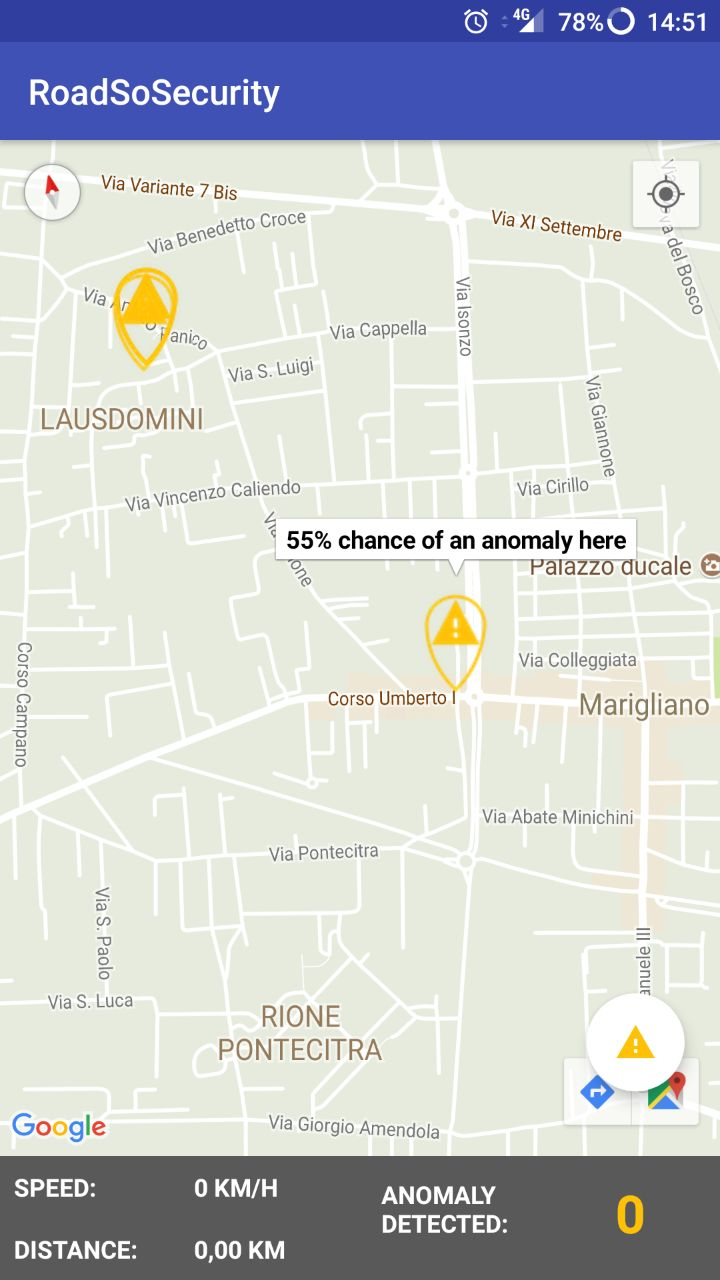
\includegraphics[width=0.38\textwidth]{images/anomalyActivity.jpg}
	\end{center}
	\caption{Activity delle anomalie stradali.}
	\label{fig:activityAnomaly}
\end{wrapfigure}

Alla fine dell'elaborazione di \textit{doInBackground(Void... arg0)} l'esecuzione del thread si sposta nel metodo \textit{onPostExecute(Void result)}, il quale aggiunge le anomalie contenute nella lista \textit{anomalyList} alla mappa. Con l'obiettivo di rendere visibili le buche stradali sulla mappa, come è possibile notare in Figura \ref{fig:activityAnomaly}, si è ciclata la lista contenente le anomalie scaricate dal web service e per ognuna di esse si è creato un marker, successivamente poi sono stati aggiunti alla mappa tramite il metodo \textit{addMarker()} utilizzando le cordinate. Inoltre ogni marker riporta il valore di fedeltà, infatti l'anomalia selezionata riportata in Figura \ref{fig:activityAnomaly} segnala la probabilità di trovare una buca stradale del $55\%$. 
Per poter lavorare con la mappa si è utilizzato le Google Maps Android API che consentono di aggiungere delle mappe ad un’applicazione senza preoccuparsi di gestire l’accesso ai server di Google, di dover scaricare le mappe e di gestire l’interazione con l’utente. 

Per utilizzare Google Maps su Android occorre ottenere un’API Key ottenibile gratuitamente sul sito ufficiale di Google e richiedere i permessi nel \textit{AndroidManifest.xml} di INTERNET; 
\begin{verbatim}
	<uses-permission android:name="android.permission.INTERNET" />
\end{verbatim}
Istanziata tramite un MapFragment, il quale consente di aggiungere una mappa in un Fragment di Android come contenitore per l’oggetto GoogleMap. Infine si è implementato l’interfaccia OnMapReadyCallback per utilizzare il metodo di callback \textit{onMapReady(GoogleMap)} per ottenere un handle all’oggetto GoogleMap in modo da poter interagire con la mappa ed inserire marker descritti in precedenza.

Inoltre è stato implementato un footer personalizzato, situato nella parte bassa dell'activity contenente la mappa \ref{fig:activityAnomaly} che indica: la velocità istantanea dell'autista, la distanza percorsa e il numero delle anomalie rilevate in maniera automatica o segnalate manualmente attraverso il \textit{FloatingActionButton}.

\subsection*{Rilevamento anomalia stradale}

In questo paragrafo verrà discusso in maniera dettagliata il processo di rilevamento delle anomalie stradali all'interno dell'applicativo.\\\\
Il front-end è stato sviluppato per essere usato all'interno dell'abitacolo del veicolo, di conseguenza il dispositivo mobile si muove rispetto al movimento del veicolo. 
Questo ci permette di monitorare il movimento del veicolo utilizzando l'accelerometro, un sensore di movimento che misura l'accelerazione sui tre assi: $X$, $Y$ e $Z$. La lettura dell'asse $Y$ indica l'accelerazione verticale del veicolo, dato che
lo smartphone è posizionato verticalmente sul cruscotto, allineando così l'asse $Y$ con quello del veicolo. Pertanto, eventuali urti di strada, buche o qualsiasi altra forma di anomalia stradale saranno riflessi come un salto nell'asse di lettura $Y$. 
\begin{figure}[h]
	\begin{center}
		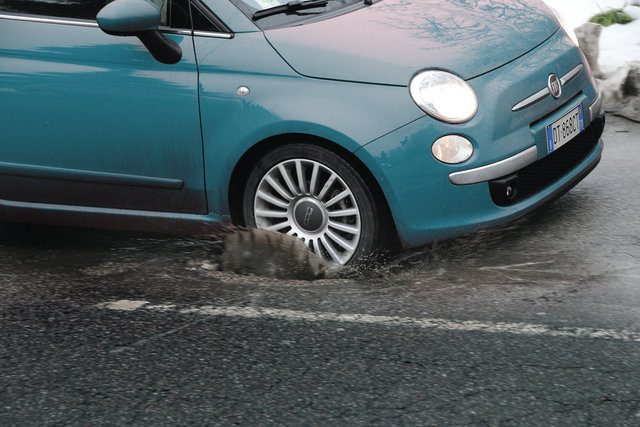
\includegraphics[width=\textwidth]{images/pothole.jpg}
	\end{center}
	\caption{Una buca stradale provoca un cambiamento sull'asse verticale nel moto del veicolo.}
	\label{fig:pothole}
\end{figure}

La Figura \ref{fig:pothole} mostra un esempio di buca stradale, in questo caso l'accelerazione del veicolo nell'asse verticale cambia creandò così un urto che viene percepito dal sensore dello smartphone. Un cambiamento di accelerazione sull'asse $Y$ superiore ad una certa soglia, viene intuito come anomalia e quindi segnalata istantaneamente attraverso un marker sulla mappa. La parte di codice che si occupa di rilevare un urto è la seguente: 
\begin{lstlisting}
@Override
public void onSensorChanged(SensorEvent event) {

double ax, ay, az;
if (event.sensor.getType() == Sensor.TYPE_ACCELEROMETER) {
 ax = event.values[0];
 ay = event.values[1];
 az = event.values[2];
 
 mAccelLast = mAccelCurrent;
 mAccelCurrent = Math.sqrt(ax * ax + ay * ay + az * az);
 double delta = mAccelCurrent - mAccelLast;
 mAccel = mAccel * 0.9f + delta;

 int temp = utility.compare((int) ax, (int) ay, (int) az);
 if (temp == 1) {
  if ((mAccelLast - mAccelCurrent) > 5) {
   if (latLng != null) {
    utility.playSound(getBaseContext(),1);
    anomalyDetectedList.add(new Anomaly(latLng.latitude, latLng.longitude));
    refreshMap();
    drawMarkerWithCircle(latLng);
   }
...
}
\end{lstlisting} 
La classe che si occupa della gestione dei sensori è android.hardware.SensorManager di cui si può ottenere un'istanza attraverso il metodo getSystemService() della classe Context (superclasse dell'Activity). Un sensore invece è rappresentato da una particolare istanza della classe android.hardware.Sensor. La classe Sensor implementa alcuni metodi, ma quello usato da noi per rilevare l'accelerometro è \textit{getType()}, il quale ritorna un intero che identifica la tipologia di sensore a cui è associato. Per accedere ai dati che il sensore rileva, l'approcio è asincrono, cioè si registra attraverso un listener ed in base ad un delay impostato manualmente, vengono notificati i valori che il sensore rileva. Per prima cosa si è implementato un listener opportuno che viene rappresentato dall'interfaccia SensorEventListener che definisce il metodo \textit{onSensorChanged(SensorEvent event)}, il quale viene invocato quando i valori del sensore cambiano. Quando il cellulare è in posizione verticale, ottenibile attraverso la funzione \textit{compare(x,y,z)} può essere rilevata una differenza di accelerazione tra due istanti $\epsilon$ superiore alla soglia impostata; solo allora viene lanciato un messaggio vocale che allerta l'autista dell'avvenuta rilevazione della buca stradale e aggiunge alla lista con la posizione ottenuta dal sensore GPS. Dopodichè viene chiamata la funzione \textit{refreshMap()} con lo scopo di aggiornare i marker sulla mappa e aumentare il contatore contenuto nel footer, inoltre viene chiamata la funzione \textit{drawMarkerWithCircle(latLng)} che delinea un cerchio di diametro $\simeq 6m$ non visibile, intorno alla nosta posizione, capace di allertare l'autista attraverso un messaggio acustico la presenza di anomalie.

Una volta che l'utente sceglie di terminare il rilevamento, alla pressione del tasto indietro, ogni anomalia individuata viene inviata al web service con i dettagli della posizione, ottenuta dal sensore GPS, attraverso la 2. risorsa (\url{http://bartlombardi-001-site1.dtempurl.com/api/Anomalies?latitude=value&longitude=value}) descritta precedentemente.
Attraverso l'uso di un \textit{AsyncTask} come per la ricezione, però questa volta per ogni anomalia rilevata durante il tragitto il metodo \textit{doInBackground(Void... arg0)} effettua tante connessioni tante quante sono le anomalie impostando la posizione nell'url. La parte di codice appena descritta è riportata seguentemente.\\

\begin{lstlisting}
private class AsyncTaskSendJson extends AsyncTask<Void, Void, Void> {

 @Override
 protected Void doInBackground(Void... arg0) {

  HttpHandler sh = new HttpHandler();
  for(Anomaly anomaly : anomalyDetectedList) {

  String url = "http://bartlombardi-001-site1.dtempurl.com/Api/Anomalies"+ "?latitude="+anomaly.getLatitude() + "&longitude="+anomaly.getLongitude();
  String jsonStr = sh.makeServiceCall(url);
  }  
 }
...
}
\end{lstlisting}
\newpage



\subsection*{RIlevamento incidente}

%----------------------------------------------------------------------------------------
%	BIBLIOGRAPHY
%----------------------------------------------------------------------------------------
\newpage
\bibliographystyle{unsrt}

\bibliography{sample}

%----------------------------------------------------------------------------------------

\end{document}